%------------------------------%
%% ✎ Dylan (V1) %%%%%%%%% ✅ %%
%% ✎ Alain (V2) %%%%%%%%% ✅ %%
%% ✎ Dylan (V3) %%%%%%%%% ✅ %%
%------------------------------%

\afterpage{%
%\afterpage{%

    % Arrière-plan introduction generale
    \AddToShipoutPictureBG*{%
\includegraphics[width=\paperwidth,height=\paperheight]{src/Figures/Arriere_plan/Arriere_plan_Introduction.jpg}
    }

% Rectangle
\AddToShipoutPictureBG*{
  \begin{tikzpicture}[remember picture,overlay]
    \node[fill=white, opacity=0.75, text width=\paperwidth, minimum height=5cm, anchor=north] 
    at ([yshift=-9cm]current page.north) {};
  \end{tikzpicture}
}

% Source
\AddToShipoutPictureFG*{
  \AtPageLowerRight{
    \raisebox{1cm}{
      \hspace{16cm}
      
\begin{tikzpicture}
        \node[fill=white, rounded corners=5pt, inner sep=5pt, align=center] {
          \tiny{Photography: \textcolor{blue}{Dylan Moinse (2024)}}
        };
      \end{tikzpicture}
    }
  }
}
}%}

\renewcommand{\thefigure}{I.\arabic{figure}} % Numérotation spécifique pour l'introduction
\renewcommand{\thetable}{I.\arabic{table}}
\setcounter{figure}{0}

\pagenumbering{arabic}
\setcounter{page}{1} % Réinitialiser la numérotation à 1

    \needspace{1\baselineskip} % Réserve de l'espace
\part*{Introduction
    \label{body:introduction-generale}
    }
    %\addcontentsline{toc}{part}{Introduction}
    \markboth{Introduction}{}
    \markright{Introduction}{}
    \begin{refsegment}

    % Citation
    \begin{displayquote}
\Commas{\textsl{Keeping in mind that~–~for the same time and effort~–~someone can cycle five times farther than they can walk, these larger catchment areas actually play a critical role in feeding more customers into the public transport system. And they may~–~at least to a certain extent~–~tamp the demand for housing in and around train stations.} [\dots] \textsl{These investments in bicycle parking, rentals, and service make perfect economic sense for public transport agencies, as they increase ridership and revenue. Rather than treating the bicycle as a competitor, it is seen as an ally~–~one that connects passengers to their origin and destination; a critical component of the seamless door-to-door journey. These kinds of collective investments in a frequent and flexible public transport system~–~to maximize its convenience and coverage~–~are precisely what governments must do to lighten the financial burden of car ownership and break down the all-too-real barriers experienced by those lowest on the socioeconomic ladder.} [\dots] \textsl{in this case, we were no longer limited by the walking distance to shops, services, and public transport; nor were we forced to compete with the high demand for such proximity. With the extended range provided by pedal power, we could suddenly open up our search to entirely new parts of the city} [\dots] \textsl{An equitable region is one that provides residents with the same access to opportunity, regardless of their postal code. With a national rail network and national cycling network at our disposal, we know we can live virtually anywhere in the Randstad, without compromising on our lifestyle and our employment opportunities. And for us, that's a great place to be.}}

\textcolor{blue}{\textcite{bruntlett_curbing_2020}}\index{Bruntlett, Melissa|pagebf}\index{Bruntlett, Chris|pagebf}. \foreignlanguage{english}{\textsl{Curbing Traffic: The Human Case for Fewer Cars in Our Lives}, Island Press, p. 164-168.}%%Rédigé%%
    \end{displayquote}

% Hook
\lettrine[lines=3, findent=8pt, nindent=0pt]{\lettrinefont G}{\textbf{etting}} \textbf{the city back on rails} (\textsl{remettre la ville sur des rails}), such is the message conveyed by filmed anthropology, produced by \textcolor{blue}{Christian} \textcolor{blue}{\textcite{lallier_ville_2010}}\index{Lallier, Christian|pagebf}, French anthropologist and filmmaker. Titled \textsl{The City on Rails. The Utopia of the Metropolis} (\textsl{La ville sur des rails. L'utopie de la métropole}), this documentary explores the challenges of rail-oriented urbanism, brought back into focus \textcolor{blue}{\autocite[8]{lhostis_concevoir_2009}}\index{L'Hostis, Alain|pagebf}\index{Alexandre, Elsa|pagebf}\index{Appert, Manuel|pagebf}\index{Araud-Ruyant, Catherine|pagebf}\index{Basty, Marius|pagebf}\index{Biau, Géraldine|pagebf}\index{Bozzani-Franc, Sandra|pagebf}\index{Boutantin, Gratienne|pagebf}\index{Constantin, Chantal|pagebf}\index{Coralli, Monica|pagebf}\index{Durousset, Marie-Jeanne|pagebf}\index{Fradier, Christophe|pagebf}\index{Gabion, Cyrille|pagebf}\index{Leysens, Thomas|pagebf}\index{Mermoud, Françoise|pagebf}\index{Olny, Xavier|pagebf}\index{Perrin, Emmanuel|pagebf}\index{Robert, Jean|pagebf}\index{Simand, Noémie|pagebf}\index{Stransky, Vaclav|pagebf}\index{Soulas, Claude|pagebf}\index{Verdier, Anne-Marie|pagebf}\index{Vulturescu, Bogdan|pagebf} with the aim of reducing car dependency \textcolor{blue}{\autocites[15]{newman_ten_2000}[74]{motte-baumvol_territoires_2014}[4]{gallez_dependance_2018}}\index{Motte-Baumvol, Benjamin|pagebf}\index{Belton-Chevallier, Leslie|pagebf}\index{Morel-Brochet, Annabelle|pagebf}\index{Gallez, Caroline|pagebf}\index{Newman, Peter W.~G.|pagebf}\index{Kenworthy, Jeffrey~R.|pagebf}. Reflections and projects related to the dialectic between network and territory, that is, the interaction between territorial logics and network logics, have recently gained momentum \textcolor{blue}{\autocite[17]{gachon_impact_2019}}\index{Gachon, Mickaël|pagebf}, in a context where their coordination is becoming an essential part of urban \Commas{Sustainable Development} discourses \textcolor{blue}{\autocite[69]{nessi_politiques_2009}}\index{Nessi, Hélène|pagebf}\index{Delpirou, Aurélien|pagebf}, mainly leading to densification around train stations. These authors, however, raise questions about the systemic ability of rail to \Commas{correct the anomalies} inherited from territorial fragmentation \textcolor{blue}{\autocite[190]{ducharme_ville_2021}}\index{Ducharme, Olivier|pagebf} and the cultural dominance of \Commas{automobility} \textcolor{blue}{\autocites[57-58]{urry_sociology_2000}[28]{urry_system_2004}}\index{Urry, John|pagebf}.%%Translated%%

% Citation
Starting from these critiques regarding the adaptability limits of the \acrshort{TOD}, or transit-oriented development, particularly in areas shaped by the car-centered system, the central hypothesis is to explore the strategic role of bicycles and \gls{micromobility}, which show a lasting trend towards a \textquote{revival} \textcolor{blue}{\autocites[137-168]{heran_retour_2015}[3-28]{dusong_dynamiques_2021}[44]{eskenazi_voir_2022}}\index{Héran, Frédéric|pagebf}\index{Dusong, Clément|pagebf}\index{Papon, Francis|pagebf}\index{Eskenazi, Manon|pagebf}\index{Massot, \index{Eskenazi, Manon|pagebf}|pagebf} or are being reinvented \textcolor{blue}{\autocite[18]{amar_homo_2016}}\index{Amar, Georges|pagebf}. The aim of this doctoral research is to assess to what extent these modes of transport can fill the gaps of the originally formulated urban planning concept, by reconfiguring the interactions between proximity, public transport, and urban forms, from an intermodal perspective. In this regard, we consider the observed rise of cycling as an opportunity to effectively address the issue of \textquote{first and last miles} of public transportation. This thesis explores, in this sense, the windfall effect of the emergence of new mobility solutions within this family of individual and light vehicles \textcolor{blue}{\autocite[77]{oostendorp_combining_2018}}\index{Oostendorp, Rebekka|pagebf}\index{Gebhardt, Laura|pagebf}, to promote \textquote{smooth and door-to-door} journeys, as accurately summarized by the quote from \textcolor{blue}{\textcite[164-168]{bruntlett_curbing_2020}}\index{Bruntlett, Melissa|pagebf}\index{Bruntlett, Chris|pagebf}.%%Translated%%

% --- %
    % *.1. Context
    \needspace{1\baselineskip} % Reserve space
\section*{Cross-Perspectives on Territorial Organization and Spatial Mobility
    \label{introduction-generale:regards-croises-organisation-territoriale-mobilite-spatiale}
    }
    \addcontentsline{toc}{section}{Cross-Perspectives on Territorial Organization and Spatial Mobility}
    %\markboth{Cross-Perspectives on Territorial Organization and Spatial Mobility}{}
    \markright{Cross-Perspectives on Territorial Organization and Spatial Mobility}{}

% Context
The transport sector remains the leading source of \acrfull{GHG} emissions in France, accounting for 32\% of total national emissions in 2022 \textcolor{blue}{\autocite[41-53]{ministere_de_la_transition_ecologique_et_de_la_cohesion_des_territoires_chiffres_2024}}\index{Ministère de la Transition Écologique et de la Cohésion des Territoires@\textsl{Ministère de la Transition Écologique et de la Cohésion des Territoires}|pagebf}. Despite a general trend towards reducing carbon footprints across the country, the transport sector saw a 2.3\% increase in its carbon emissions over the year. This rise is mainly attributable to the use of private cars, which are responsible for more than half of these emissions, despite the frequent promises of technical and technological solutions. The unrestrained use of \textquote{auto-centrism} fits into a vicious cycle of automobile dependency, where European urban growth since the post-war period has been persistently shaped by its adaptation to the widespread use of cars. This process has led to the fragmentation of spaces, longer travel distances, and the structuring of networks, urban forms, and land uses, creating territorial vulnerabilities. As a result, the paradigm of \textquote{sustainable mobility} or \textquote{mobility transition} and, more broadly, its \textquote{decarbonization}, is primarily a matter of urban planning \textcolor{blue}{\autocite{societe_francaise_des_urbanistes_decarbonation_2024}}\index{Société française des urbanistes@\textsl{Société française des urbanistes}|pagebf}. In this sense, the train station district serves as a strategic junction between the city and transport, drawing the focus of urban planners. To \textquote{reweave} the city, public transport must be seen as the structural element of corridors and neighborhoods, a pivot from which urban development actors are invited to rethink the organization of territories \textcolor{blue}{\autocite[8]{boisclair_retisser_2013}}\index{Boisclair, Catherine|pagebf}.%%Translated%%

% TOD
Rising to the level of an action reference, the issue of coordination between urban planning and transport, beyond the \textquote{myth of coherence}, introduces the theoretical and operational model of \acrfull{TOD} \textcolor{blue}{\autocite[183-220]{gallez_mythes_2010}}\index{Gallez, Caroline|pagebf}\index{Kaufmann, Vincent|pagebf}\index{Guerrinha, Christophe|pagebf}\index{Maksim, Hanja-Niriana|pagebf}\index{Thébert, Mariane|pagebf}, in which the technical object and its environment interact in co-construction over time \textcolor{blue}{\autocite[44-50]{leheis-guillot_ville_2011}}\index{Leheis-Guillot, Stéphanie|pagebf}. This integrated approach, which involves simultaneously thinking about the city and transport, relies on a mechanism of bidirectional and continuous interaction, embedded in a feedback loop \textcolor{blue}{\autocite[130]{wegener_overview_2004}}\index{Wegener, Michael|pagebf}. It is within this systemic framework that we support the hypothesis that \acrshort{TOD} would benefit from better integrating the proximities generated by train station districts, both in terms of flow polarization and urban insertion opportunities. Just like the title chosen by the British researcher \textcolor{blue}{Rich~C.} \textcolor{blue}{\textcite[40]{mcilroy_this_2023}}\index{McIlroy, Rich~C.|pagebf}, in his article \textsl{This is where public transport falls down}\footnote{
    \textsl{This is where public transport falls down} \textcolor{blue}{\autocite[40]{mcilroy_this_2023}}\index{McIlroy, Rich~C.|pagebf}.
}, the primary challenge of \acrshort{TOD} today is less about improving the quality of public transport and intensifying human activities around exchange hubs, than it is about enhancing the pathways to and from these nodes. In short, while hopes for decarbonizing mobility focus on the \textquote{magic triptych} – composed of the car, whether electric, shared, autonomous, or connected – it seems likely that this focus on the automobile, whose rebound effects and persistent nuisances are underestimated, will prove insufficient. Conversely, the focus should be on the synergy between walking, \gls{bicycle}, and public transport, a more fitting \textquote{intermodal triptych} capable of addressing contemporary urban mobility challenges and territorial planning \textcolor{blue}{\autocite[1]{soulas_triptyque_2021}}\index{Soulas, Claude|pagebf}.%%Translated%%

% Light Individual Mobility + Research Topic
The urban model of \acrshort{TOD} aims to link two distinct scales of daily mobility: on one hand, metropolitan and regional mobility, structured by public transport networks, and on the other hand, proximity mobility, which prioritizes walking and cycling as much as possible \textcolor{blue}{\autocites[81]{conesa_modelisation_2010}[124]{lo_feudo_scenario_2014}}\index{Lo Feudo, Fausto|pagebf}\index{Menerault, Philippe|pagebf}\index{L'Hostis, Alain|pagebf}\index{Festa, Demetrio Carmine|pagebf}\index{Conesa, Alexis|pagebf}\index{Paris, Didier|pagebf}. However, over the last decade, bicycles and micromobility have diversified to the point that they tend to \textquote{hybridize}, evolving into individual, transportable objects \textcolor{blue}{\autocite[20]{amar_du_2012}}\index{Amar, Georges|pagebf}, such as \acrfull{PeS}, or resembling individual public transport systems \textcolor{blue}{\autocites[179]{amar_homo_2010}[4]{castex_prise_2017}}\index{Castex, Élodie|pagebf}\index{Frère, Séverine|pagebf}\index{Groux, Annette|pagebf}\index{Amar, Georges|pagebf}, similar to shared mobility. Through innovation processes driving socio-spatial transformations \textcolor{blue}{\autocite[89]{ageron_intermodalite-voyageurs_2013}}\index{Ageron, Pierre|pagebf}\index{Varlet, Jean|pagebf}, what we call \textquote{light individual mobility} is integrated into the public transport network as a complementary modal offer. Its intermodal uses are intrinsically linked to temporal and spatial dimensions, leading us to develop a reflection informed by references to spaces, territories, and places \textcolor{blue}{\autocite[4]{sebban_complementarite_2003}}\index{Sebban, Annie-Claude|pagebf}\index{Motte, Alain|pagebf}. It is from these considerations that we have established our research topic, entitled:
    \begin{displayquote}
\textbf{The Transit-Oriented Development Urban Model Revisited by Emerging Light Individual Mobility. An Investigation in the Hauts-de-France Region.}
    \end{displayquote}%%Translated%%

% --- %
    % *.2. Scientific Positioning
    \needspace{1\baselineskip} % Reserve space
\section*{Scientific Positioning
    \label{introduction-generale:positionnement-scientifique}
    }
    \addcontentsline{toc}{section}{Scientific Positioning}
    %\markboth{Scientific Positioning}{}
    \markright{Scientific Positioning}{}

% Train Station
This thesis adopts a planning approach, mobilizing elements from the \textquote{urban fabric} with a specific focus on the materiality of public spaces. As a general hypothesis, we adopt the concept of \textquote{networked urbanism} or \textquote{city of networks} as the analytical framework, considered as explanatory models of urban transformations \textcolor{blue}{\autocite[]{dupuy_urbanisme_1991}}\index{Dupuy, Gabriel|pagebf}. This framework is based on the assumption that territorial organization, made possible by networks, offers a multiplicity of connections, the optimization of which is a condition for its effectiveness. In this regard, the train station is considered as a \textquote{territorial object} \textcolor{blue}{\autocite[7]{moretti_interconnexion_1999}}\index{Moretti, Anna|pagebf}\index{Vacheret, Guy|pagebf}, a space at the interface of transport networks and urban dynamics. This concept aligns with a recent trend in urban studies aiming to reconsider the role of train stations in the structuring of contemporary cities, a \textquote{return of train stations in urban studies} \textcolor{blue}{\autocite[489]{delage_gare_2013}}\index{Delage, Aurélie|pagebf}. Far from being reduced to a mere functional connection point, the train station is viewed here in all its complexity as a \textquote{station-system} \textcolor{blue}{\autocites[395]{le_bot_quel_2019}{le_bot_management_2020}}\index{Le Bot, Nils|pagebf}. This stance integrates its spatial, organizational, and symbolic dimensions, recognizing its structuring role not only for transport networks but also for urban production and organization, as well as the lifestyles associated with it. Furthermore, the research topic is framed as transcending scales \textcolor{blue}{\autocite[3]{knowles_transit_2019}}\index{Knowles, Richard~D.|pagebf}\index{Ferbrache, Fiona|pagebf}, promoting the interlocking of temporal and scalar scales; from land and economic evolution to urban projects; from the local scale of the building-passenger to regional and (inter)national dimensions \textcolor{blue}{\autocites[13-14]{menerault_gares_2001}[238]{chapelon_transports_2016}}.%%Translated%%

% Proximities
This reflection on the train station cannot be dissociated from the mobilities it polarizes. As such, this research involves a shift in analysis, moving from the train station object to the geographical proximities it generates, incorporating a reflection on light individual mobility and its role in the structuring of train station districts. This shift in focus is part of a broader paradigmatic change in mobility analysis, to which the train station actively contributes \textcolor{blue}{\autocite[53]{leheis-guillot_ville_2011}}\index{Leheis-Guillot, Stéphanie|pagebf}. This \textquote{mobility turn} \textcolor{blue}{\autocites{sheller_new_2006}[8]{sheller_mobilizing_2016}[13]{randell_no_2020}}\index{Sheller, Mimi|pagebf}\index{Urry, John|pagebf}\index{Randell, Richard|pagebf} emphasizes the relational and systemic dimension of the \gls{journey}, beyond a strictly infrastructural approach \textcolor{blue}{\autocite[14]{heran_retour_2015}}\index{Héran, Frédéric|pagebf}. In this framework, this thesis sits at the intersection of several research fields, combining urban planning, territorial development, geography, sociology, and data science, in order to question the reconfiguration of \acrshort{TOD} under the effect of (new) proximities made possible by the integration of light individual mobility. This approach leads to considering this mobility as a strategic lever for the revitalization of \acrshort{TOD} in urban contexts inherited from the car-oriented model \textcolor{blue}{\autocite[209]{heran_retour_2015}}\index{Héran, Frédéric|pagebf}. It is thus part of a broader reflection on the renewal of public transport and urban planning policies, in the face of the challenges of the \textquote{first and last miles}. It highlights the opportunity that light individual mobility represents for promoting a multimodal and \textquote{door-to-door} mobility system \textcolor{blue}{\autocite[979]{lee_bicycle-based_2016}}\index{Lee, Jaeyeong|pagebf}\index{Choi, Keechoo|pagebf}\index{Leem, Yountaik|pagebf}.%%Translated%%

% Positioning
This doctoral research thus mobilizes four complementary approaches to structure our investigation: (i) the approach through technical objects, by analyzing the \textquote{station-system} and the associated modes of transport; (ii) the approach through uses and intermodal practices, by studying the modal behaviors and strategies of cycling passengers; (iii) the approach through \gls{accessibility}, by measuring the effects of light individual mobility on accessibility; and (iv) the approach through urban systems, by questioning the effects of light individual mobility on railway urban planning. Thus, the train station cannot be reduced to a purely socio-technical object \textcolor{blue}{\autocite[]{joseph_villes_1999}}\index{Joseph, Isaac|pagebf}, but must also be considered as an urban object, taking into account its territorial integration, beyond the scale of the building-passenger or its immediate environment. It plays a spatial, functional, and symbolic role, acting both as a \textquote{stage} and an \textquote{actor} \textcolor{blue}{\autocite[5]{baron_gares_2016}}\index{Baron, Nacima|pagebf}\index{Roseau, Nathalie|pagebf}. This approach thus allows for exploring the potential for revising \acrshort{TOD} through the integration of light individual mobility. It offers a renewed perspective on train station districts and their role in urban organization, while contributing to the formalization of an expanded model: an \acrfull{M-TOD}, or a transit-oriented development model that integrates light individual mobility.%%Translated%%

% --- %
    % *.3. Research Directions
    \needspace{1\baselineskip} % Reserve space
\section*{Research Directions
    \label{introduction-generale:problematique-objectifs-hypotheses}
    }
    \addcontentsline{toc}{section}{Research Directions}
    %\markboth{Research Problem, Objectives, and Hypotheses}{}
    \markright{Research Problem, Objectives, and Hypotheses}{}

% Research Problem
This thesis aims to examine the transformations of the \acrshort{TOD} model from the perspective of light individual mobility, adopting a theoretical, empirical, and forward-looking approach to determine and establish an optimal framework for \gls{intermodal accessibility}. Our central question is framed as follows:
    \begin{displayquote}
\textbf{To what extent can the integration of light individual mobility address the challenges of the \textquote{first and last miles} of public transport and contribute to enhancing the intermodal accessibility of train station districts in the Hauts-de-France region? \\
How do these \textquote{proximities} reconfigure the urban model of \textsl{Transit-Oriented Development} and pave the way for a \textsl{Micromobility-friendly Transit-Oriented Development}, better suited to urban realities and evolving mobility practices? \\
What are the conditions for implementation and the levers of action to be mobilized to ensure optimal integration of light individual mobility into urban planning and transport strategies?}
    \end{displayquote}%%Translated%%

% Objectives
This line of questioning will guide the structure of our research, showing how light individual mobility can enrich the \acrshort{TOD} model and the implications this has for mobility and territorial planning. Throughout our doctoral project, we will develop a progressive approach in several stages, designed to revisit the \acrshort{TOD} in light of the proximities renewed by the development of light individual mobility. Each chapter is based on a research objective, articulating both theoretical and empirical reflections on the challenges of intermodal accessibility (see the \hyperref[fig-introduction:objectifs-hypotheses]{diagram~\ref{fig-introduction:objectifs-hypotheses}}, page~\pageref{fig-introduction:objectifs-hypotheses}). To structure our reasoning, we use the \acrfull{QQOQCCP} questioning method, which allows us to clarify the contours and objectives of our research:
        \begin{customitemize}
    \item \textsl{What} and \textsl{When}? ({\textcolor{blue}{\(O_1\)}\label{objectif-1}}). The first chapter lays the conceptual and historical foundations of \acrshort{TOD} and cycling, identifying their strengths and limitations. It aims to introduce the essential nature of an \acrshort{M-TOD}, that is, a revised model that takes into account this intermodal component;
    \item \textsl{By whom} and \textsl{On what}? ({\textcolor{blue}{\(O_2\)}\label{objectif-2}}). The second chapter aims to build an analytical framework by reviewing existing scientific and technical works on light individual mobility, \gls{intermodality}, and the rethinking of \acrshort{TOD}. It puts international experiences and new knowledge on intermodality into perspective;
    \item \textsl{Where} and \textsl{With what}? ({\textcolor{blue}{\(O_3\)}\label{objectif-3}}). The third chapter uses mixed methods to construct and analyze empirical data within a defined geographical area. It aims to define, adapt, and relate appropriate approaches to propose a \textquote{custom survey};
    \item \textsl{Who} and \textsl{How many}? ({\textcolor{blue}{\(O_4\)}\label{objectif-4}}). The fourth chapter measures and characterizes intermodal practices, focusing on the profiles of users who combine the use of light individual mobility and public transport. It aims to quantify the flows and identify the socio-demographic and environmental factors influencing such modal choices;
    \item \textsl{Where to} and \textsl{Why}? ({\textcolor{blue}{\(O_5\)}\label{objectif-5}}). The fifth chapter aims to measure and explain the spatial extension of train station districts through light individual mobility. It evaluates the accessibility gains at different scales;
    \item \textsl{How} and \textsl{In relation to what}? ({\textcolor{blue}{\(O_6\)}\label{objectif-6}}). The final chapter proposes a conceptual and operational formalization of the \acrshort{M-TOD} by modeling the conditions for its implementation. It aims to formulate recommendations for urban development stakeholders.
        \end{customitemize}%%Translated%%

% Figure research objectives and hypotheses
    \begin{figure}[h!]\vspace*{4pt}
        \caption{Overview of Research Objectives and Hypotheses}
        \label{fig-introduction:objectifs-hypotheses}
        \centerline{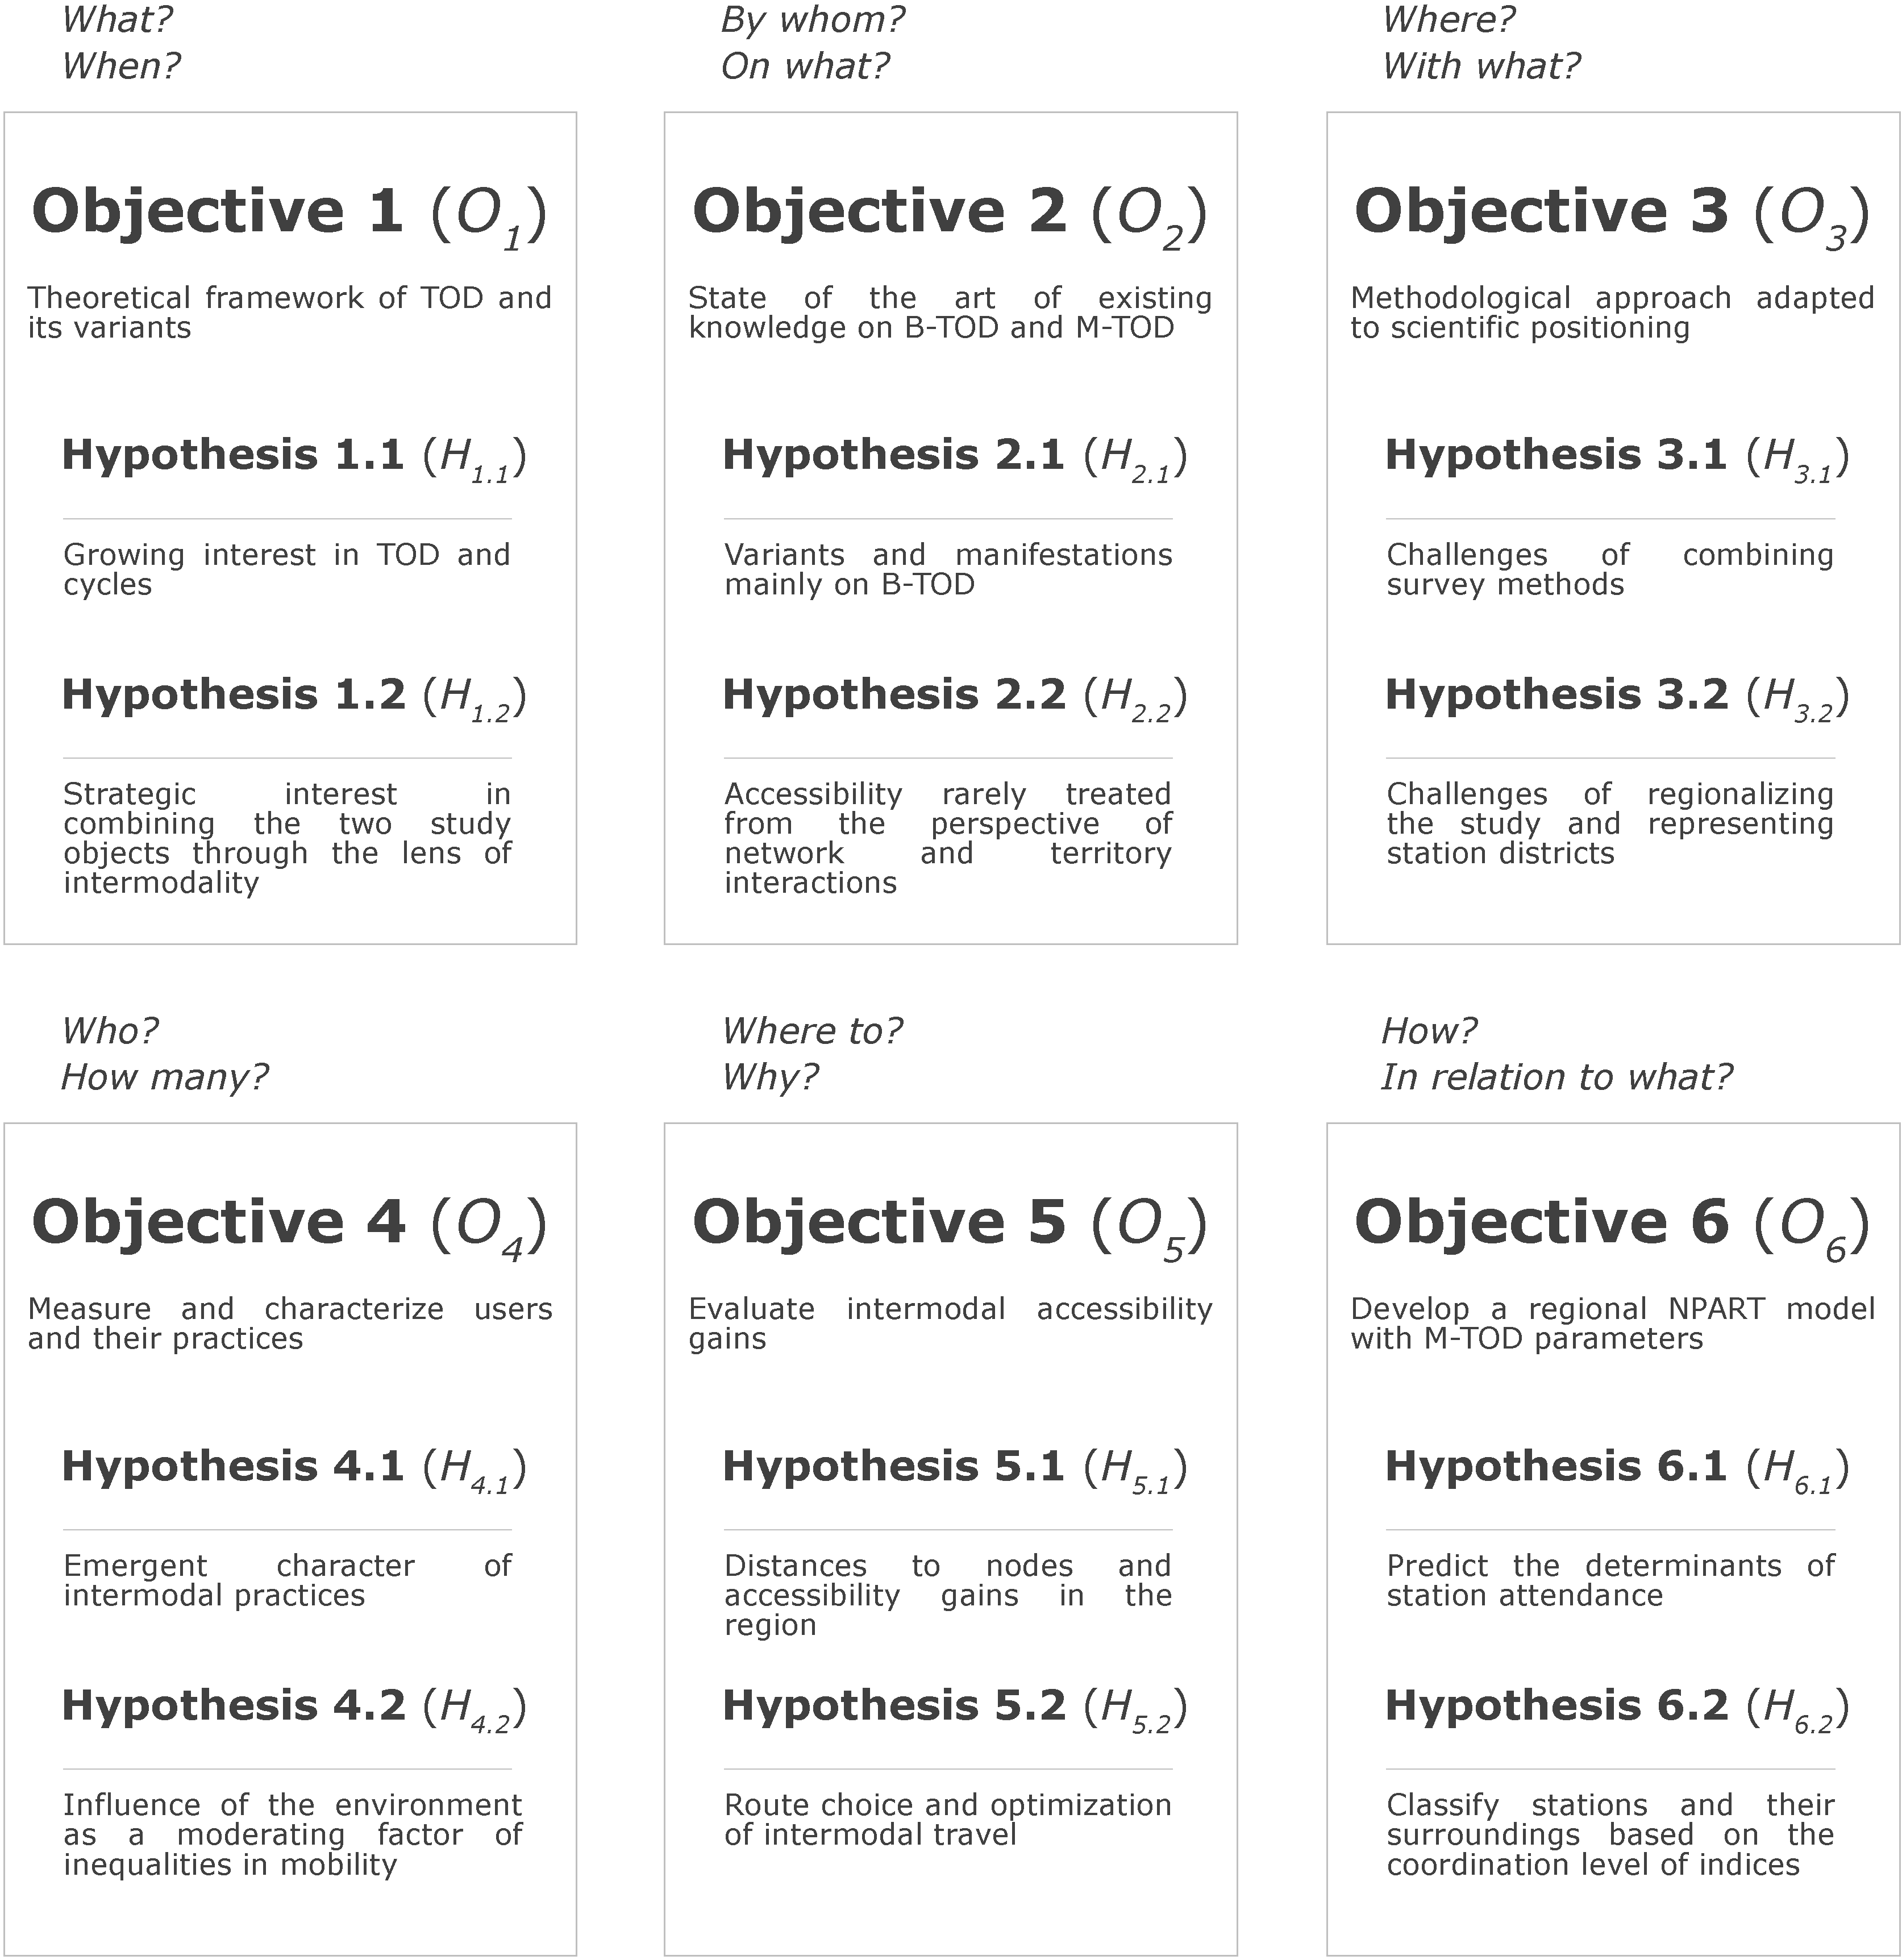
\includegraphics[width=1\columnwidth]{src/Figures/Introduction/EN_Objectifs_recherche.pdf}}
        \vspace{5pt}
        \begin{flushright}\scriptsize{
        Author~: \textcolor{blue}{Dylan Moinse (2023)}
        }\end{flushright}
    \end{figure}

% Hypotheses
Based on the previously defined objectives, which structure the various chapters of this thesis, the research hypotheses emerge, constituting the thread of our argument throughout this scientific work (see the \hyperref[fig-introduction:objectifs-hypotheses]{diagram~\ref{fig-introduction:objectifs-hypotheses}}, page~\pageref{fig-introduction:objectifs-hypotheses}). These hypotheses are based on a hypothetico-deductive approach and are characterized by their associative, complex, and directional nature\footnote{
    According to \textcolor{blue}{\textcite[41-43]{tomini_methodes_2020}}\index{Tomini, Luca|pagebf}\index{Wintgens, Sophie|pagebf}, in their handbook \textsl{Méthodes d'enquêtes de terrain en sciences sociales}, associative hypotheses postulate an interactive relationship between concepts; complex hypotheses, on the other hand, specify a relationship between multiple concepts; while directional hypotheses formulate the orientation of the links that connect these concepts.
} \textcolor{blue}{\autocite[43]{tomini_methodes_2020}}\index{Tomini, Luca|pagebf}\index{Wintgens, Sophie|pagebf}. Based on these objectives, we propose the following hypotheses to guide our reflection:
        \begin{customitemize}
    \item \textsl{Emerging research themes related to \textsl{Transit-Oriented Development} and light individual mobility deserve to be considered jointly} ({\textcolor{blue}{\(H_1\)}\label{hypothese-1}}). Indeed, both of these axes are attracting growing interest in both academic and operational spheres ({\textcolor{blue}{\(S.H_{1.1}\)}\label{sous-hypothese-1.1}}) and would benefit from being studied in an articulated manner to reveal their potential synergies ({\textcolor{blue}{\(S.H_{1.2}\)}\label{sous-hypothese-1.2}})~;
    \item \textsl{Current knowledge on this intermodal synergy remains strongly conditioned by the bicycle and train combination, and is rarely analyzed through the lens of \textsl{Transit-Oriented Development}} ({\textcolor{blue}{\(H_2\)}\label{hypothese-2}}). Existing work primarily focuses on the bicycle object ({\textcolor{blue}{\(S.H_{2.1}\)}\label{sous-hypothese-2.1}}), while accessibility issues are mostly addressed from a strictly transport-related perspective ({\textcolor{blue}{\(S.H_{2.2}\)}\label{sous-hypothese-2.2}})~;
    \item \textsl{Understanding the complexity of intermodal dynamics and their implications on the urban environment faces the challenge of defining an analytical methodology} ({\textcolor{blue}{\(H_3\)}\label{hypothese-3}}). Given the gaps identified in the literature, it seems relevant to employ a mixed-methods approach, combining various survey techniques ({\textcolor{blue}{\(S.H_{3.1}\)}\label{sous-hypothese-3.1}}). Moreover, adopting a regional study area and redefining the concept of train station districts in line with the principles of \acrshort{TOD} are necessary adjustments ({\textcolor{blue}{\(S.H_{3.2}\)}\label{sous-hypothese-3.2}})~;
    \item \textsl{Intermodal practices are experiencing significant growth due to the combined emergence of new mobility solutions, although these practices are marked by differentiated appropriation across various social groups} ({\textcolor{blue}{\(H_4\)}\label{hypothese-4}}). The development of intermodality involving cycling and public transport is part of a diversification and appropriation process of mobility modes ({\textcolor{blue}{\(S.H_{4.1}\)}\label{sous-hypothese-4.1}}). However, this appropriation remains uneven, with certain social groups adopting these modes more easily than others, a situation that could be mitigated through territorial planning interventions ({\textcolor{blue}{\(S.H_{4.2}\)}\label{sous-hypothese-4.2}})~;
    \item \textsl{Integrating light individual mobility within public transport networks is a major lever for improving regional accessibility} ({\textcolor{blue}{\(H_5\)}\label{hypothese-5}}). This integration increases the reach of trips, extending the service areas of train station districts and facilitating access to destinations ({\textcolor{blue}{\(S.H_{5.1}\)}\label{sous-hypothese-5.1}}). Additionally, it promotes the optimization of routes, making intermodal travel more competitive compared to car use, including for long-distance daily mobility ({\textcolor{blue}{\(S.H_{5.2}\)}\label{sous-hypothese-5.2}})~;
    \item \textsl{Expanding the concept of urban planning to include light individual mobility is a lever for revitalizing train station districts, enhancing their accessibility in a broader sense} ({\textcolor{blue}{\(H_6\)}\label{hypothese-6}}). Certain factors related to the cyclability of train station districts help stimulate demand around exchange hubs ({\textcolor{blue}{\(S.H_{6.1}\)}\label{sous-hypothese-6.1}}), while making them more consistent with the guiding principles of \acrshort{TOD} ({\textcolor{blue}{\(S.H_{6.2}\)}\label{sous-hypothese-6.2}}).
\end{customitemize}%%Translated%%

% --- %
    % *.4. Methodology
    \needspace{1\baselineskip} % Reserve space
\section*{Research Strategy
    \label{introduction-generale:methodologie}
    }
    \addcontentsline{toc}{section}{Research Strategy}
    %\markboth{Methodology}{}
    \markright{Methodological Framework}{}

% Introduction
In order to address the research problem and the formulated objectives and hypotheses, this thesis adopts a mixed methodological approach, combining original methods tailored to the specifics of the subject under study (see the \hyperref[fig-introduction:methodes-hypotheses]{diagram~\ref{fig-introduction:methodes-hypotheses}}, page~\pageref{fig-introduction:methodes-hypotheses}). This methodological approach enables the articulation of three essential dimensions: (i) a conceptual reflection on the evolution of \acrshort{TOD} and its relationship with light individual mobility; (ii) an investigation into existing intermodal practices and the factors influencing these mobility behaviors; and (iii) an assessment of the effects of light individual mobility on accessibility to train stations and on the structuring of surrounding districts, within a regional scope. Far from being a linear approach, this methodological path embraces its complexity, mobilizing complementary tools in order to capture the multiple dimensions of \acrshort{TOD} and light individual mobility, in accordance with the \hyperref[hypothese-3]{hypothesis~\(H_3\)} (page~\pageref{hypothese-3}).%%Translated%%

% Figure methodology hypotheses
    \begin{figure}[h!]\vspace*{4pt}
        \caption{Methodological Framework Designed in Dialogue with the Research Hypotheses}
        \label{fig-introduction:methodes-hypotheses}
        \centerline{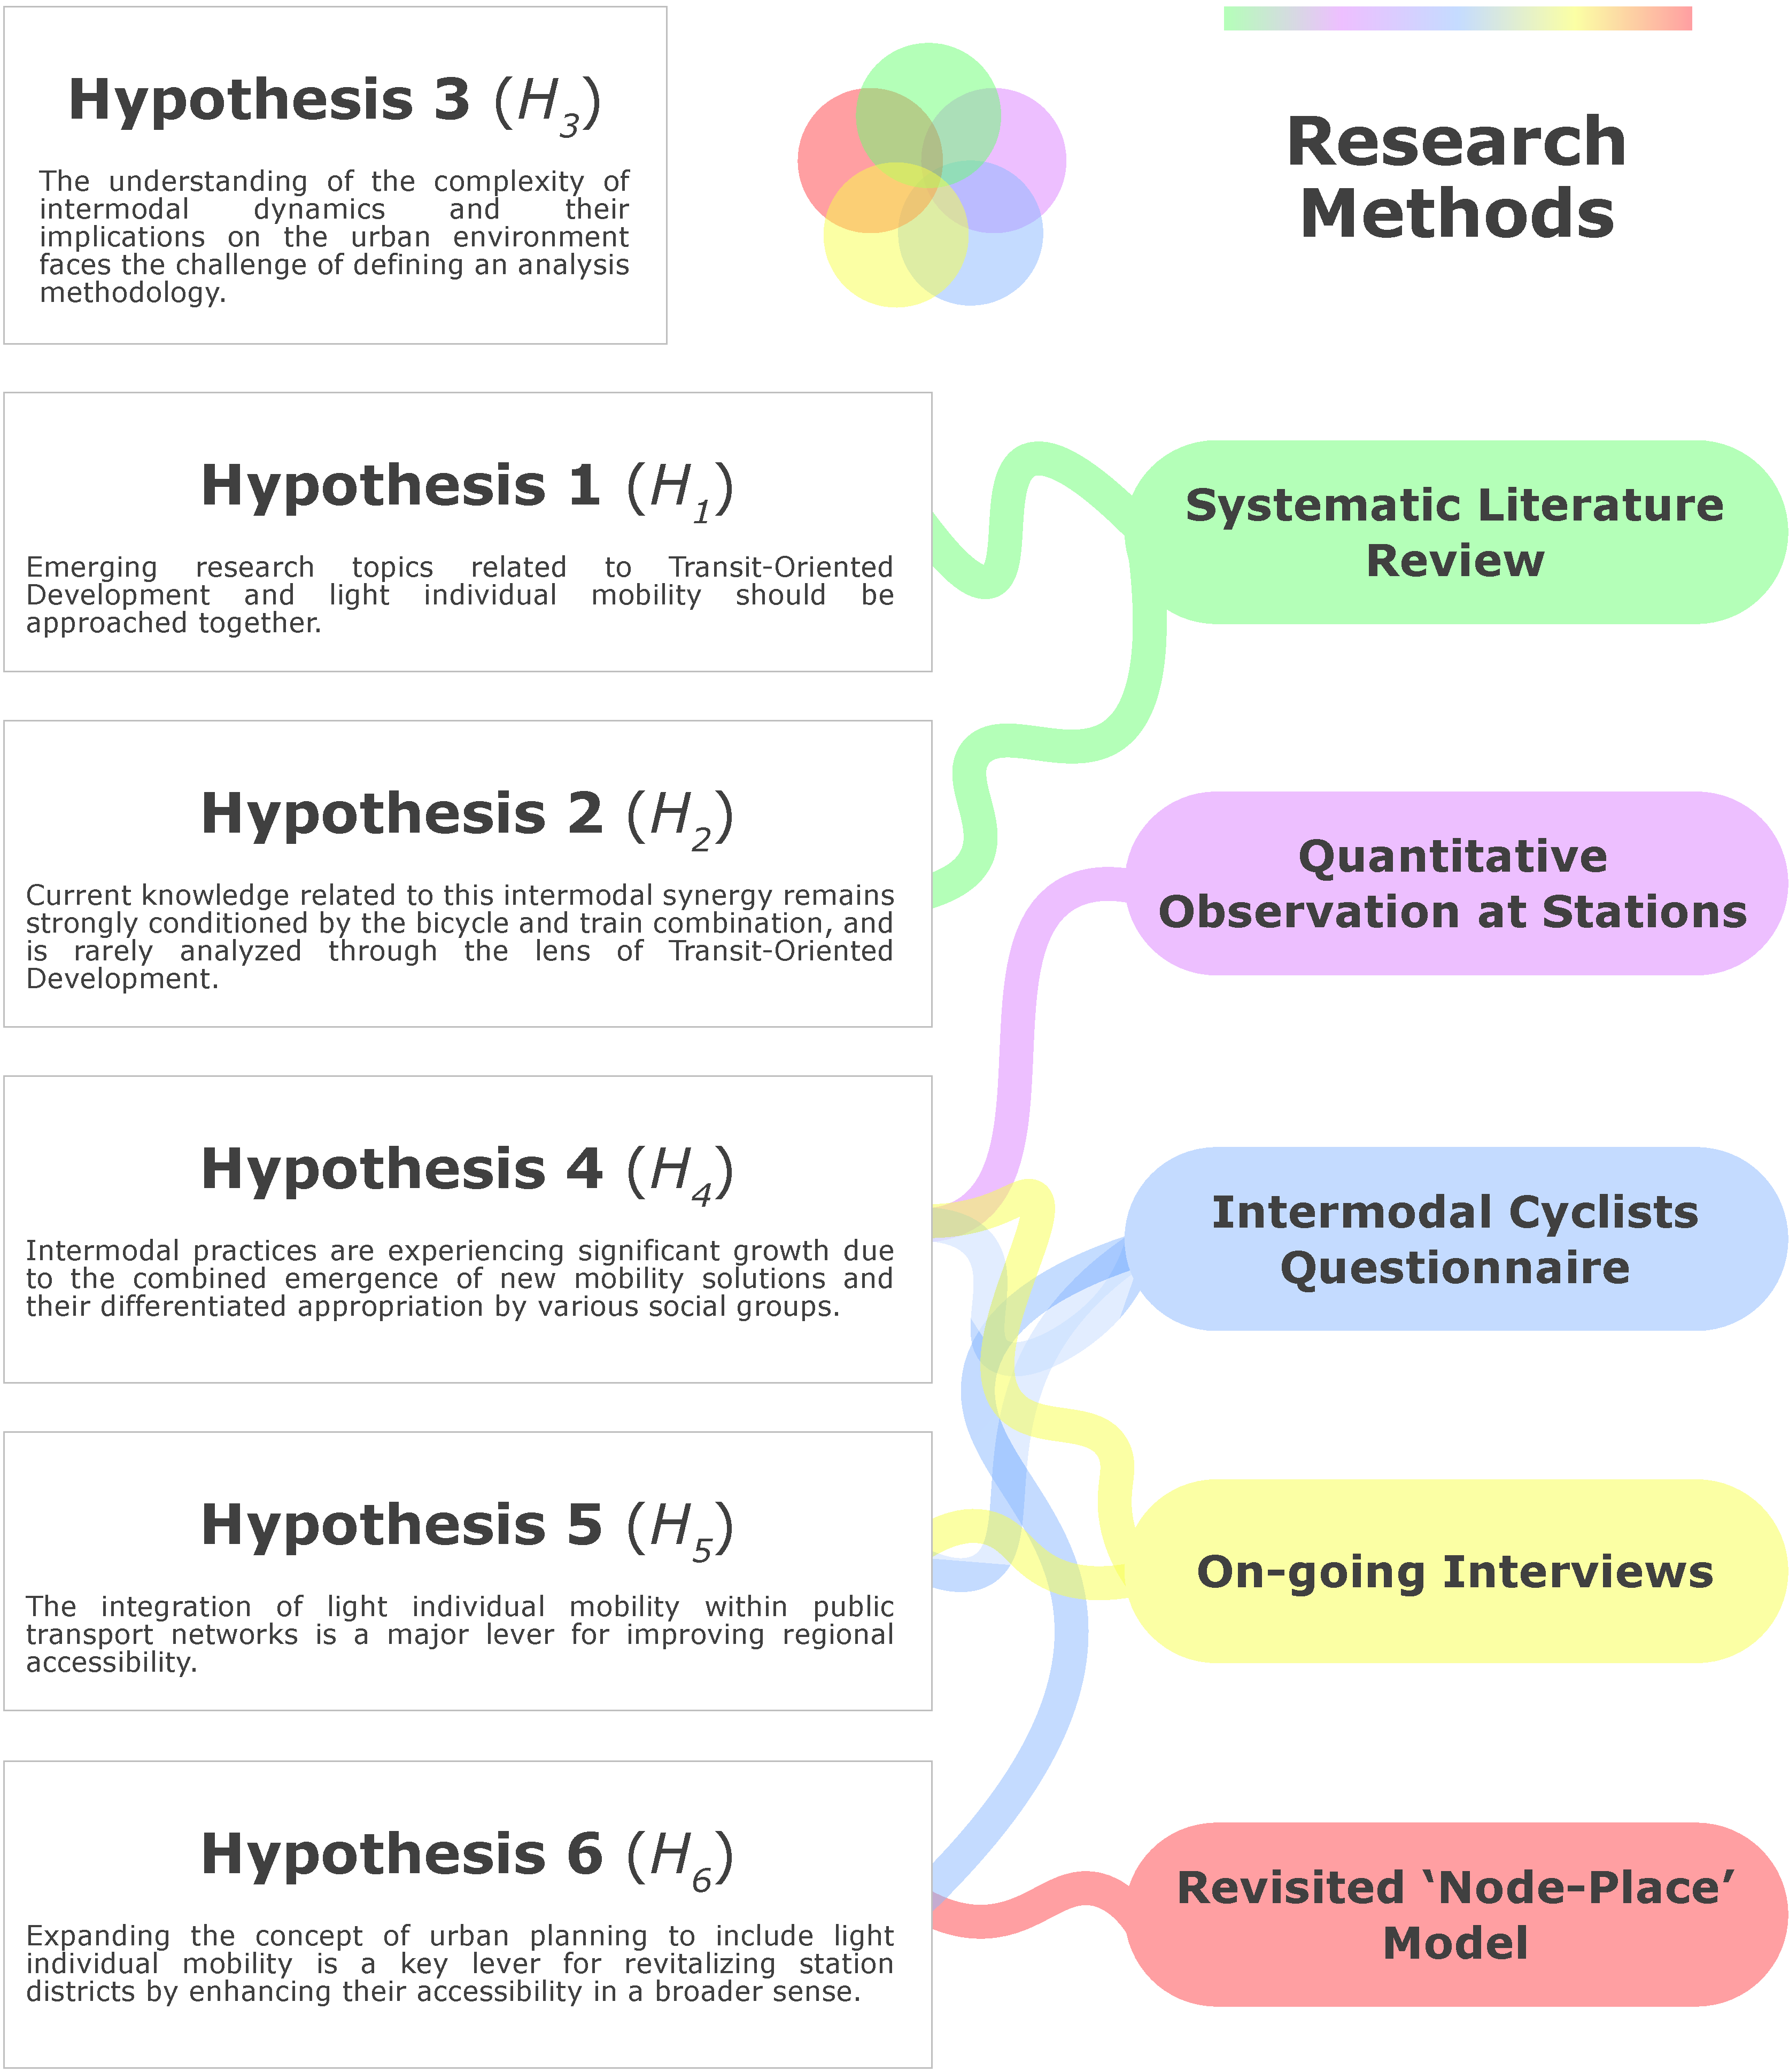
\includegraphics[width=1\columnwidth]{src/Figures/Introduction/EN_Methodologie_hypotheses.pdf}}
        \vspace{5pt}
        \begin{flushright}\scriptsize{
        Author~: \textcolor{blue}{Dylan Moinse (2025)}
        }\end{flushright}
    \end{figure}

% Methodology
The chosen methodology is primarily based on the need to synthesize existing works and knowledge related to the research problem. To this end, a \acrfull{SLR} was conducted on studies related to the contours of \acrshort{B-TOD} and \acrshort{M-TOD}, in line with \hyperref[hypothese-1]{hypotheses~\(H_1\)} and \hyperref[hypothese-2]{\(H_2\)} (page~\pageref{hypothese-2}). This is followed by field exploration in the form of a quantitative observation, aimed at characterizing the emerging phenomenon of nodal connection facilitated by light individual mobility, in accordance with \hyperref[hypothese-4]{hypothesis~\(H_4\)} (page~\pageref{hypothese-4}). This survey is complemented by conducting mobile interviews, with a guided route, enriching the investigation by accessing the \gls{perception} of users and refining the understanding of their intermodal practices. A third type of survey involves a questionnaire addressed to cycling passengers, intended to represent intermodal travel in order to identify the territories frequented and experienced near exchange hubs, continuing from \hyperref[hypothese-5]{hypothesis~\(H_5\)} (page~\pageref{hypothese-5}). Finally, spatial modeling has been undertaken to revisit the \textquote{node-place} tool, commonly applied in \acrshort{TOD} studies. This modeling allows for capturing the implications of integrating light individual mobility and identifying its interactions with the urban environment, supported by \hyperref[hypothese-6]{hypothesis~\(H_6\)} (page~\pageref{hypothese-6}).%%Translated%%

% --- %
    % *.5. Thesis Outline
    \needspace{1\baselineskip} % Reserve space
\section*{Thesis Structure
    \label{introduction-generale:annonce-plan}
    }
    \addcontentsline{toc}{section}{Thesis Structure}
    %\markboth{Thesis Outline}{}
    \markright{Thesis Outline}{}

% Introduction
This thesis is structured into three parts and six chapters, following a logical progression that allows for the exploration of the theoretical foundations, challenges, and implications of integrating light individual mobility into the \acrshort{TOD} model (see the \hyperref[fig-introduction:structure-these]{diagram~\ref{fig-introduction:structure-these}}, page~\pageref{fig-introduction:structure-these}). Alternating between conceptual approach, state of the art, methodological framework, empirical study, and prospective modeling, it leads to the proposal of a renewed model: an \acrfull{M-TOD}. The argument developed is based on three main axes: (i) a deep understanding of the uses and behaviors related to light individual mobility from an intermodal perspective; (ii) a multi-criteria analysis of the potential for accommodating territories based on their capacity to integrate these new forms of mobility; and (iii) an inquiry into the role of public action in planning and structuring these practices within transport and urban policies. In parallel, three progressive and multiscalar levels of analysis underpin this reflection: (i) examining the dynamics of intermodal demand; (ii) evaluating intermodal accessibility, considered from the perspective of network performance, available resources, time constraints, and individual characteristics; (iii) as well as analyzing the interactions between transport and urban planning in a context of modal integration. The structure of this research, which reflects the scientific approach adopted, can be summarized as follows: \textsl{synthesize and rethink} (see \hyperref[part1:titre]{Part One}, page~\pageref{part1:titre}); \textsl{represent and understand} (see \hyperref[part2:titre]{Part Two}, page~\pageref{part2:titre}); and \textsl{anticipate and guide} (see \hyperref[part3:titre]{Part Three}, page~\pageref{part3:titre}).%%Translated%%

% Figure structure of the thesis
    \begin{figure}[h!]\vspace*{4pt}
        \caption{Overall Structure of the Doctoral Research}
        \label{fig-introduction:structure-these}
        \centerline{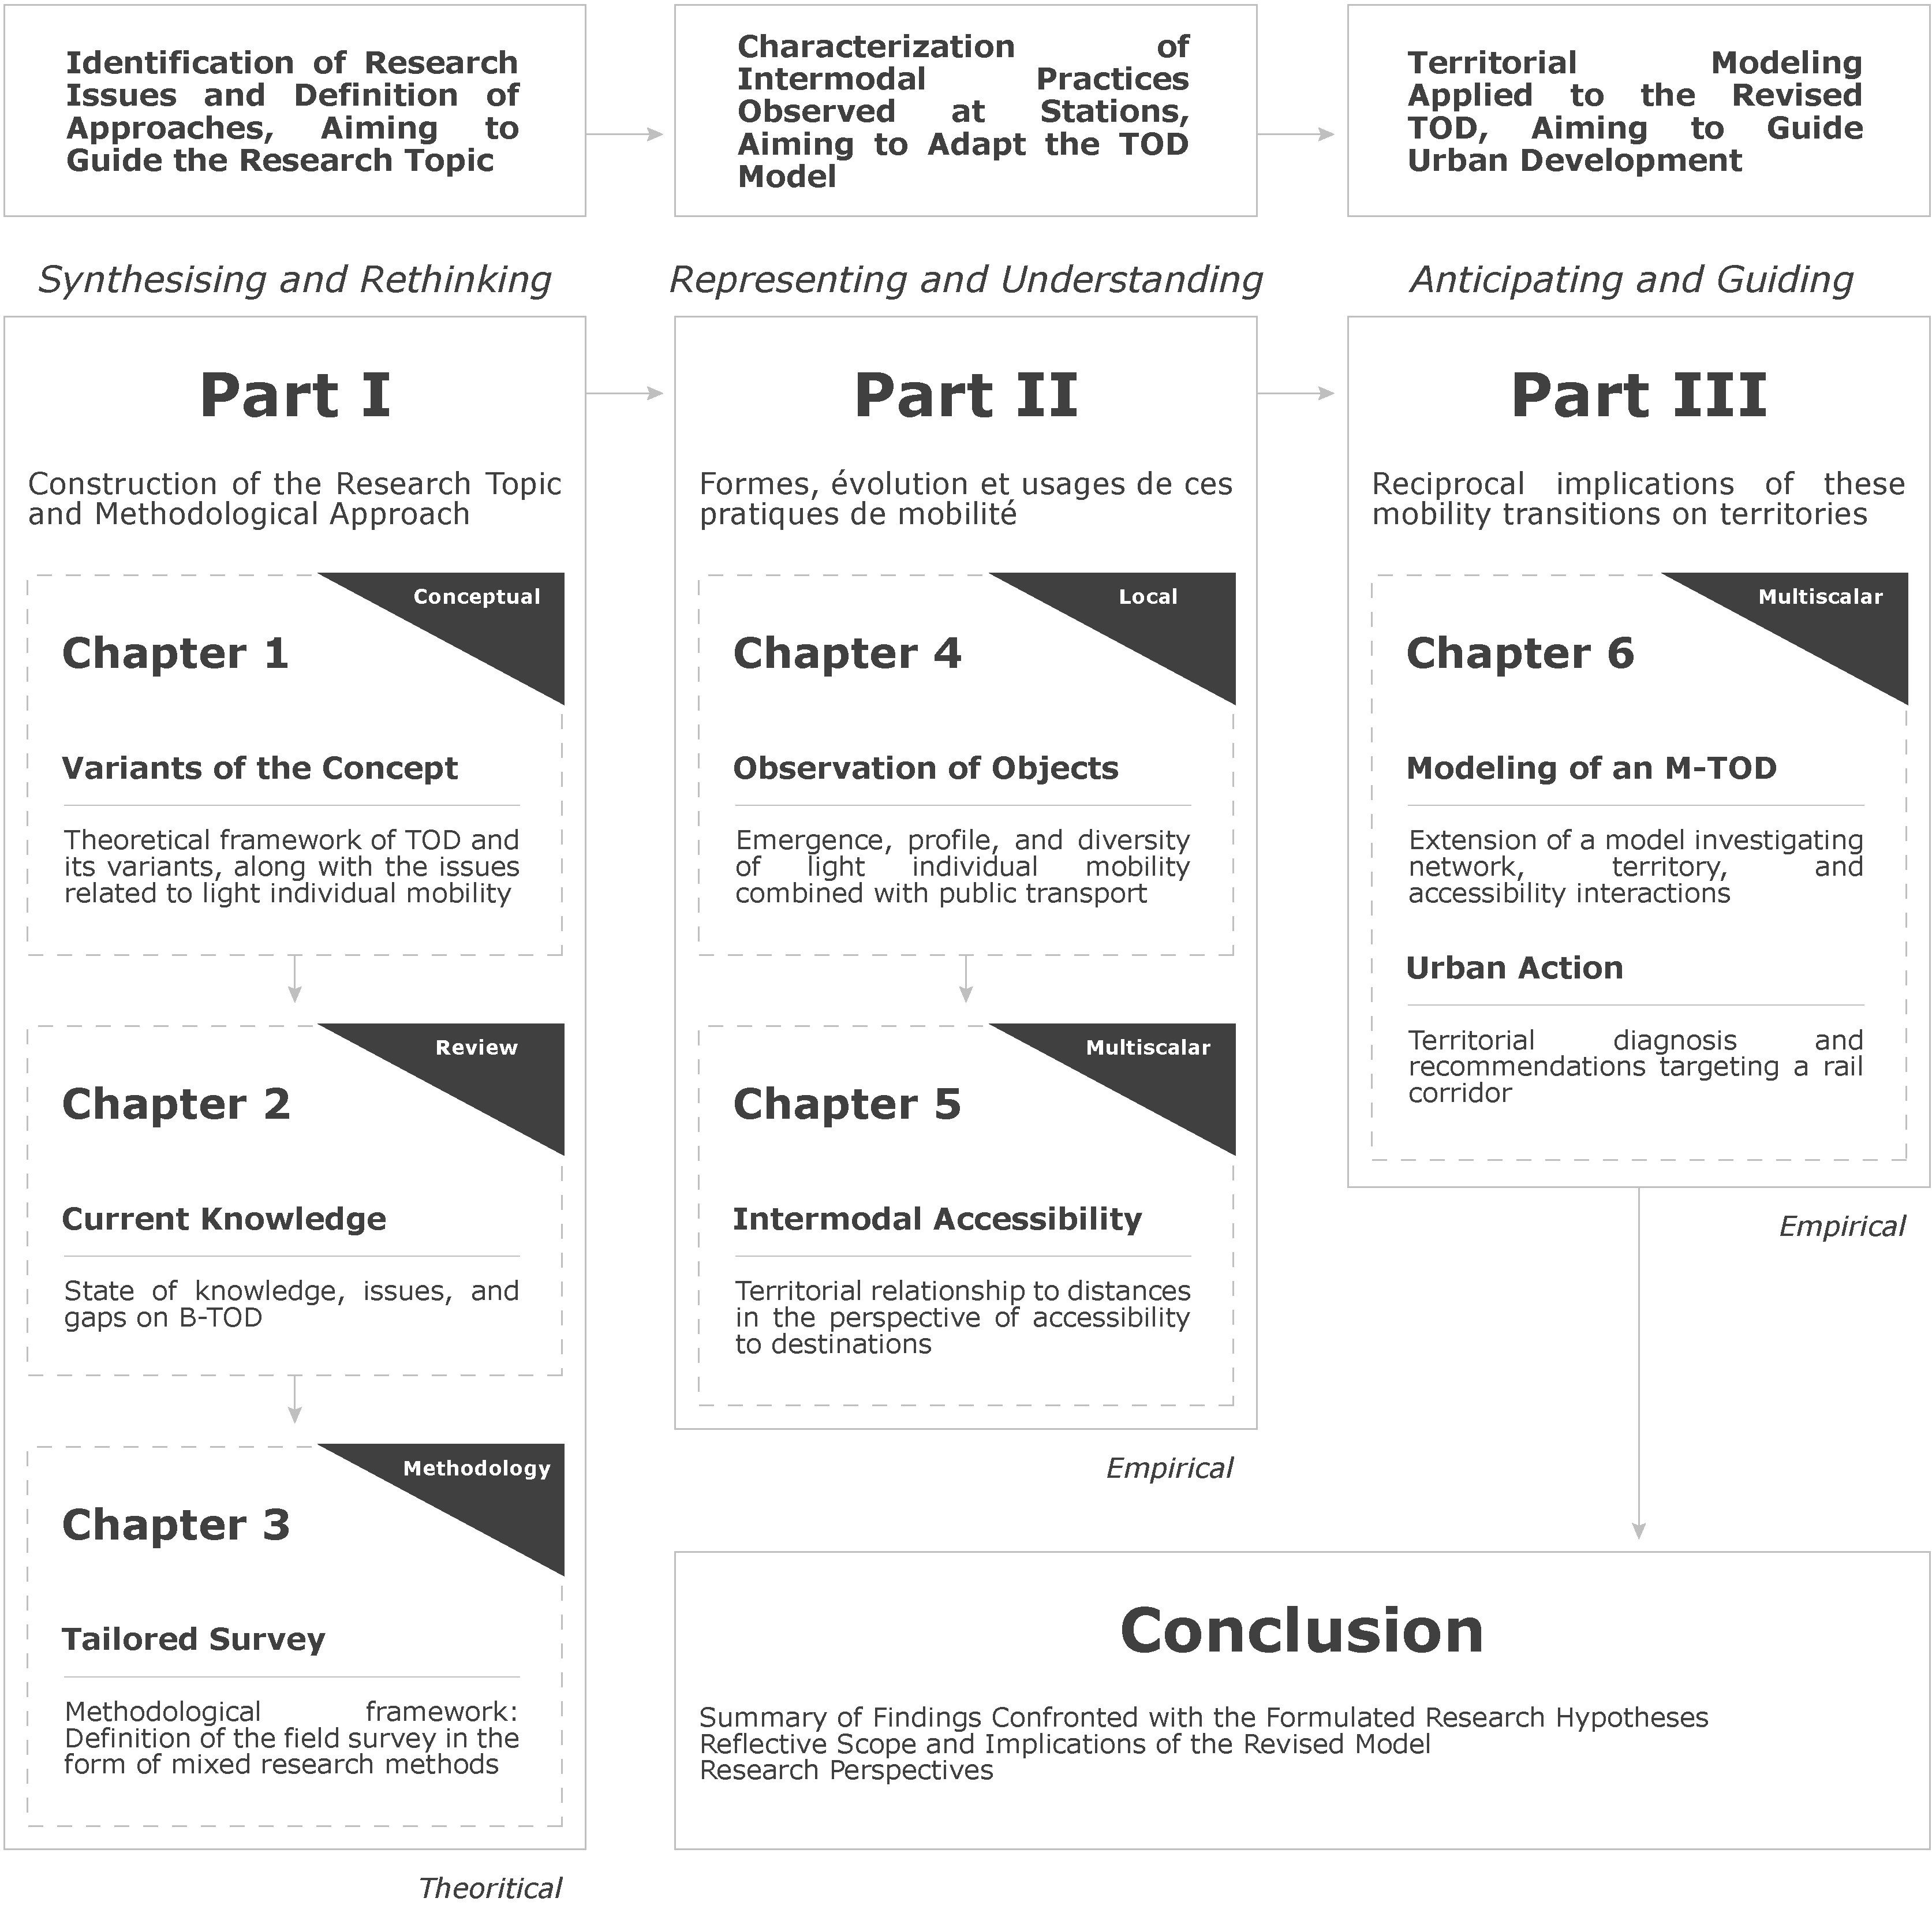
\includegraphics[width=1\columnwidth]{src/Figures/Introduction/EN_Structure_these.pdf}}
        \vspace{5pt}
        \begin{flushright}\scriptsize{
        Author~: \textcolor{blue}{Dylan Moinse (2023)}
        }\end{flushright}
    \end{figure}

% *.5.1. Outline of the plan: part 1
    \needspace{1\baselineskip} % Reserve space
\subsection*{Part One: \textsl{Synthesize and Rethink}
    \label{introduction-generale:annonce-plan-1}
    }

% Chapter 1
\hyperref[chap1:titre]{Chapter One} (page~\pageref{chap1:titre}) lays the theoretical foundations of this research by defining the fundamental concepts that will structure the argument. It first focuses on the founding principles of \acrshort{TOD}, tracing its evolution and various conceptual and operational adaptations. This urban planning model, conceived as an alternative to the car-centered system, aims to structure urbanization around public transport infrastructures. However, its application reveals limitations in certain contexts, particularly in peri-urban areas where access distances to public transport stations constitute a major barrier to its effectiveness. It is from this perspective that the analysis of light individual mobility is positioned, defined here as a set of vehicles including bicycles and their variants, as well as scooters and other means of transport. These solutions emerge as a strategic lever capable of addressing the shortcomings of conventional \acrshort{TOD} by improving accessibility to hubs, in the context of the \textquote{first and last miles} of public transport. This chapter thus explores the rise of cycling in daily mobility and its gradual inclusion in urban planning policies. It then examines the opportunities associated with integrating light individual mobility into \acrshort{TOD} thinking, questioning its implications in terms of geographical proximity and intermodality. Finally, it concludes with a critical review of the literature, highlighting the theoretical gaps and potentials of an expanded model that incorporates these new intersections between mobility and urban planning, which justify the investigation undertaken in this thesis (\hyperref[objectif-1]{objective~\(O_1\)}, page~\pageref{objectif-1}).%%Translated%%

% Chapter 2
\hyperref[chap2:titre]{Chapter Two} (page~\pageref{chap2:titre}) extends the reflection initiated on the evolution of \acrshort{TOD} by delving deeper into the state of knowledge on its adaptations incorporating light individual mobility, particularly \acrshort{B-TOD} and \acrshort{M-TOD}. It provides a state of the art on the interaction between bicycles, micromobility, and public transport, questioning these interactions at the interface of mobility systems and territorial organization. Drawing on a \acrfull{SLR}, this chapter employs a scientometric approach to identify the geographical, temporal, and institutional dynamics structuring these urban planning models. This study supports the recent rise in research dedicated to these themes and the emergence of new methodological tools, particularly the use of \textsl{Big Data} and geostatistical analysis models. It identifies the key urban determinants influencing mobility behaviors and evaluates the accessibility gains induced by integrating light individual mobility into \acrshort{TOD} strategies. Based on these elements, this chapter defines the theoretical and methodological foundations upon which the empirical investigation conducted in the following chapters rests (\hyperref[objectif-2]{objective~\(O_2\)}, page~\pageref{objectif-2}).%%Translated%%

% Chapter 3
\hyperref[chap3:titre]{Chapter Three} (page~\pageref{chap3:titre}) marks the entry into the study field of the thesis by seeking to evaluate the integration of light individual mobility into the urban model. It presents the methodological framework adopted to carry out this investigation. This chapter contributes to a reflection on the epistemological positioning of the research, justifying the adoption of mixed research methods, combining quantitative and qualitative approaches. This methodology allows for understanding the complexity of mobility behaviors as well as their relationships and effects on territorial accessibility, by cross-referencing different sources of information. This approach, describing the methodological choices, data collection and processing tools, and the construction of the study areas, lays the analytical foundation that guides the interpretation of the results in the following sections (\hyperref[objectif-3]{objective~\(O_3\)}, page~\pageref{objectif-3}).%%Translated%%

% *.5.2. Outline of the plan: part 2
    \needspace{1\baselineskip} % Reserve space
\subsection*{Part Two: \textsl{Represent and Understand}
    \label{introduction-generale:annonce-plan-2}
    }

% Chapter 4
\hyperref[chap4:titre]{Chapter Four} (page~\pageref{chap4:titre}) constitutes the first phase of the empirical analysis, focusing on the study of intermodal practices associated with light individual mobility, which are found in train station districts. It aims, on the one hand, to quantify the extent of the phenomenon by measuring the modal share of transfer modes in travel chains involving public transport. On the other hand, it seeks to better define the corpus of cycling passengers and identify the key factors influencing their modal choices, considering their individual characteristics, perceptions, and their relationship to the urban environment. This chapter highlights the trade-offs made by users in their daily organization of intermodal travel and emphasizes the role of territorial arrangements as structuring factors of these emerging practices. It identifies the conditions that favor their growth and thus prepares the spatial analysis of the next chapter, questioning the role of accessibility and urban configurations as catalysts for these behaviors (\hyperref[objectif-4]{objective~\(O_4\)}, page~\pageref{objectif-4}).%%Translated%%

% Chapter 5
Based on the exploratory results obtained, \hyperref[chap5:titre]{Chapter Five} (page~\pageref{chap5:titre}) focuses on the accessibility gains generated by these modal synergies. It examines how these intermodal practices transform access to train stations and contribute to the reconfiguration of surrounding districts by redefining the influence areas of transport nodes. The main objective is to assess the contribution of light individual mobility in extending the service areas of public transport stops, as well as the benefits in terms of regional access to destinations. The projection of the routes taken highlights the preferred pathways and the factors influencing these choices. This reflection leads to a renewed interpretation of the functional boundaries of train station districts, showing how the integration of light individual mobility can alter their spatial organization and enhance their attractiveness as strategic locations (\hyperref[objectif-5]{objective~\(O_5\)}, page~\pageref{objectif-5}).%%Translated%%

% *.5.3. Outline of the plan: part 3
    \needspace{1\baselineskip} % Reserve space
\subsection*{Part Three: \textsl{Anticipate and Guide}
    \label{introduction-generale:annonce-plan-3}
    }

% Chapter 6
\hyperref[chap6:titre]{Chapter Six} (page~\pageref{chap6:titre}) proposes a formalization of the \acrshort{M-TOD}, designed as an extension of the \acrshort{TOD} that fully integrates the geographical proximities promised by the combined use of walking and light individual mobility. Based on the insights gained, this chapter engages in modeling the \acrshort{M-TOD}, in order to define its guiding principles, its implementation conditions, and the levers to activate in order to promote its development and maximize its benefits. The proposed modeling particularly allows for predicting the patronage of train stations based on the territorial arrangements of each train station district examined, and the pedestrian and cycling accessibility scales within the regional area studied. A classification of the train stations and their service areas is then established, allowing for the identification of strategic urban hubs with the potential for implementing \acrshort{TOD} and \acrshort{M-TOD}, as well as those for which investments and improvements should be considered to strengthen their role in a global alternative mobility system. Finally, this chapter opens with the production of a territorial diagnosis, formulating a series of strategic recommendations, applied to a case study focusing on a railway corridor (\hyperref[objectif-6]{objective~\(O_6\)}, page~\pageref{objectif-6}).%%Translated%%

    % ___________________________________________
    % Subbibliography
    \newpage
    \sectionheader{Bibliography of Introduction}
    \begingroup
    \renewcommand{\bibfont}{\scriptsize}
\printbibliography[segment=\therefsegment, heading=subbibintoc, title={Bibliography of Introduction}, label=introduction:bibliographie]
    \endgroup
    \end{refsegment}